\documentclass[12pt]{article}
\usepackage[brazil]{babel}
\usepackage{design_ASC}
\usepackage{enumitem}
\usepackage{subfig}
\usepackage{gensymb}

\setlength\parindent{0pt} %% Do not touch this

%% -----------------------------
%% TITLE
%% -----------------------------
\title{Prova 1} %% Assignment Title

\author{Victor F. Ferrari\\ %% Student name
MO814A/MC937A - Tópicos in Computação Gráfica\\ %% Code and course name
\textsc{Universidade Estadual de Campinas}
}

\date{\today} %% Change "\today" by another date manually
%% -----------------------------
%% -----------------------------

%% %%%%%%%%%%%%%%%%%%%%%%%%%
\begin{document}
\setlength{\droptitle}{-5em}    
%% %%%%%%%%%%%%%%%%%%%%%%%%%
\maketitle

% --------------------------
% Start here
% --------------------------

% %%%%%%%%%%%%%%%%%%%
\section*{Questão 1}
% %%%%%%%%%%%%%%%%%%%
{\bfseries Explique o \textit{pipeline} de visualização em um sistema gráfico. Quais suas etapas?}

\textit{Nota: tive 3 interpretações desse enunciado. Tenho certa certeza de que a resposta 1 é a desejada, mas se não for, incluí mais 2 respostas de interpretações diferentes. Creio que não sejam necessárias.}

\textbf{Resposta 1: pipeline de uma representação gráfica para a exibição ao usuário.}

Em um sistema gráfico, a imagem se inicia com seus pontos em OCS, coordenadas do objeto. O objetivo é transformar esses pontos para coordenadas do mundo, depois para coordenadas de visão, e finalmente para coordenadas da \textbf{janela} de exibição.

Assim, a primeira etapa é a transformação para \textbf{WCS}, coordenadas da cena, que podem ser diferentes das coordenadas de um objeto. Em seguida, se realiza a transformação para as \textbf{coordenadas de visão}, o que normalmente consiste em transformações projetivas. Por último, é feita a conversão para coordenadas da janela de exibição (\textit{viewport}), chamadas de \textbf{DCS}. É nessa etapa que ocorre o \textit{clipping} de polígonos e retas, e enfim a imagem está pronta para exibição: a cena foi transformada em uma imagem a ser exibida.

\bigskip
\textbf{Resposta 2: pipeline de um sistema de visão computacional.}

Se o sistema tem uma percepção do ambiente que precisa ser interpretado, o processo inicia com a \textbf{aquisição} da imagem com uma câmera digital ou outro dispositivo, representando a cena a ser "vista". Então, a imagem pode ser \textbf{pré-processada} inteiramente para melhorar a qualidade da entrada. Isso leva à fase de \textbf{processamento}, na qual apenas as informações importantes para a aplicação são filtradas e limpas para melhor análise (por exemplo, extraindo bordas de objetos e filtrando ruído).

A imagem então passa por \textbf{análise}, que depende da aplicação em questão (por exemplo, identificar bifurcações e terminais em impressões digitais). Esses pontos de interesse são então modelados por \textbf{extração de características} (por exemplo, combinar múltiplos pontos identificados geometricamente), e finalmente usados para \textbf{reconhecimento de padrões}, comparando a estrutura final com entradas anteriores ou uma referência armazenada.

\bigskip
\textbf{Resposta 3: etapas para visualização de dados.}

Se o sistema não tem percepção, e quer apenas oferecer uma visualização de dados para o usuário, o sistema passa por uma fase de análise dos dados, para extrair informações interessantes para a aplicação, em seguida uma etapa de agregação e modelamento desses dados em gráficos e outras estruturas gráficas. Finalmente, essa estrutura final é exibida ao usuário.

% %%%%%%%%%%%%%%%%%%%
\section*{Questão 2}
% %%%%%%%%%%%%%%%%%%%
{\bfseries Como você definiria as seguintes cores em RGB, CMY e HSV?

\begin{enumerate}[label=\alph*)]
    \item Uma cor vermelho pura
    \item Uma cor lilás
    \item Amarelo
    \item Marrom
    \item Como é dada a equivalência entre os modelos RGB, CMY e HSV?
\end{enumerate}
}

\textbf{a)}

A cor vermelho é dada diretamente pelo modelo RGB, por ser uma cor básica do modelo.

\bigskip
\begin{itemize}
    \item RGB: (255, 0, 0): maior valor possível em vermelho, e os menores valores possíveis em verde e azul.
    \item CMY: $\begin{pmatrix}1 & 1 & 1\end{pmatrix} - \frac{\begin{pmatrix}255 & 0 & 0\end{pmatrix}}{255}$ = (0, 1, 1), normalizado. De 0 a 100, temos (0, 100, 100).
    \item HSV:
\end{itemize}{}

Começamos com RGB normalizado para (1,0,0).
\begin{gather*}
V = \max(RGB) = 1 \\
C = V-\min(RGB) = V = 1.\\
\end{gather*}
Como V é igual a R:
\begin{gather*}
H = 60*\frac{(G-B)}{C} = 60*0 = 0\\
S = \frac{C}{V} = 1\\
\end{gather*}

Assim, \textbf{HSV = (0, 1, 1)}

\bigskip
\textbf{b)}

A cor lilás, no modelo RGB, tem valores (200, 162, 200).

\bigskip
\begin{itemize}
    \item RGB: (200, 162, 200).
    \item CMY: $\begin{pmatrix}1 & 1 & 1\end{pmatrix} - \frac{\begin{pmatrix}200 & 162 & 200\end{pmatrix}}{255}$ = (0.2157, 0.3647, 0.2157), normalizado. De 0 a 100, temos (21.57, 36.47, 21.57). O lilás é uma cor que se beneficia do modelo CMYK, consistindo apenas de magenta e K (preto), porém no modelo CMY as outras cores são usadas para se obter o preto.
    \item HSV:
\end{itemize}{}

Começamos com RGB normalizado para (0.78431373, 0.63529412, 0.78431373).
\begin{gather*}
V = \max(RGB) = 0.78431373 \\
C = V-\min(RGB) = V-G = 0.149\\
\end{gather*}
Como V é igual a B:
\begin{gather*}
H = 60*(4+\frac{(R-G)}{C}) = 60*(4+1) = 300\\
S = \frac{C}{V} = 0.19\\
\end{gather*}

Assim, \textbf{HSV = (300, 0.19, 0.7843)}

\bigskip
\textbf{c)}

A cor amarelo é dada diretamente pelo modelo CMY, por ser uma cor básica do modelo.

\bigskip
\begin{itemize}
    \item CMY: (0, 0, 100): maior valor possível em amarelo, e os menores valores possíveis em magenta e ciano.
    \item RGB: $\begin{pmatrix}1 & 1 & 1\end{pmatrix} - \frac{\begin{pmatrix}0 & 0 & 100\end{pmatrix}}{100}$ = (1, 1, 0), normalizado. De 0 a 255, temos (255, 255, 0). 
    \item HSV:
\end{itemize}{}

Começamos com RGB normalizado para (1, 1, 0).
\begin{gather*}
V = \max(RGB) = 1 \\
C = V-\min(RGB) = V = 1\\
\end{gather*}
Como V é igual a R:
\begin{gather*}
H = 60*\frac{(G-B)}{C} = 60*1 = 60\\
S = \frac{C}{V} = 1\\
\end{gather*}

Assim, \textbf{HSV = (60, 1, 1)}

\bigskip
\textbf{d)}

A cor marrom, no modelo RGB, tem valores (150, 75, 0).

\bigskip
\begin{itemize}
    \item RGB: (150, 75, 0).
    \item CMY: $\begin{pmatrix}1 & 1 & 1\end{pmatrix} - \frac{\begin{pmatrix}150 & 75 & 0\end{pmatrix}}{255}$ = (0.4118, 0.7059, 1), normalizado. De 0 a 100, temos (41.18, 70.59, 100).
    \item HSV:
\end{itemize}{}

Começamos com RGB normalizado para (0.58823529, 0.29411765, 0).
\begin{gather*}
V = \max(RGB) = 0.58823529 \\
C = V-\min(RGB) = V = 0.58823529\\
\end{gather*}
Como V é igual a R:
\begin{gather*}
H = 60*\frac{(G-B)}{C} = 60*0.5 = 30\\
S = \frac{C}{V} = 1\\
\end{gather*}

Assim, \textbf{HSV = (30, 1, 0.5882)}

\bigskip
\textbf{e)} RGB e CMY são modelos complementares, ou seja, ciano é a cor complementar (ou secundária) de vermelho, magenta é a cor complementar de verde, e amarelo é a cor complementar de azul. Assim, RGB é um modelo aditivo (soma das cores é branco) e CMY é um modelo subtrativo (soma das cores é preto), sendo tão ligados que basta tomar o inverso dos valores de um modelo para atingir o outro. Ambos se baseiam na teoria tricromática.
    
Já o modelo HSV se baseia em outras características de cor: a matiz, a luminosidade e a saturação. Sendo fundamentalmente diferente, a relação com os outros dois não é direta, e sim algorítmica. Esse algoritmo se baseia em modelar o HSV como um cone/pirâmide, em vez do cubo RGB (que também inclui CMY). Nessa pirâmide de seis lados, cada vértice da base corresponde a uma das cores dos outros modelos vistos, o centro da base é a cor branca e o vértice da pirâmide é a cor preta. A altura representa o "valor" (V), que é a luminosidade, o ângulo a partir do centro é a matiz (H), e a distância do centro é a saturação (S).

% %%%%%%%%%%%%%%%%%%%
\section*{Questão 3}
% %%%%%%%%%%%%%%%%%%%
{\bfseries Dados os seguintes polígonos:

\begin{figure}[H]
    \centering
    \subfloat[Polígono A]{
    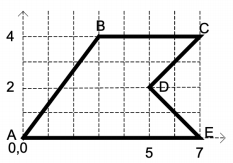
\includegraphics{images/3/3a.png}
    \label{fig:3a}
    }
    \subfloat[Polígono B]{
    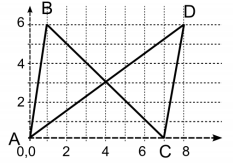
\includegraphics{images/3/3b.png}
    \label{fig:3b}
    }
    \caption{Polígonos}
\end{figure}{}

\begin{enumerate}[label=\alph*)]
    \item Para o polígono A: Mostre como fica a AET para as linhas de varredura 0 a 4 e quais pixéis são desenhados em cada interação do algoritmo de preenchimento de polígonos.
    \item Para o polígono B: Mostre como fica a AET para as linhas de varredura 0 a 6 e quais pixels são desenhados em cada interação do algoritmo de preenchimento de polígonos.
\end{enumerate}
}

\textbf{a)}

A AET do polígono A pode ser vista na figura \ref{fig:3a_aet}.
\begin{figure}[H]
    \centering
    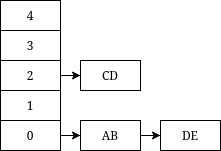
\includegraphics[width=0.3\textwidth]{images/3/3a_aet.png}
    \caption{AET do polígono A}
    \label{fig:3a_aet}
\end{figure}

A cada iteração do algoritmo, se tem uma AEL (\textit{Active Edge List}), a partir da qual são calculados os pixels a serem desenhados. Para cada iteração (ou seja, \textit{scanline}), temos um diagrama da AEL correspondente, e cada iteração desenha pixels na imagem com uma cor específica. No texto, os pixels indicados são os valores em X, como o valor em Y é o mesmo para cada iteração.

\begin{itemize}
    \item Linha 0: pixels 0-6 (amarelo).
\begin{figure}[H]
    \centering
    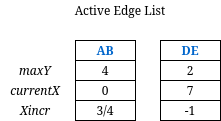
\includegraphics[width=0.4\textwidth]{images/3/3a_ael0.png}
    \caption*{AEL na linha 0.}
\end{figure}
    \item Linha 1: pixels 1-5 (vermelho).

\begin{figure}[H]
    \centering
    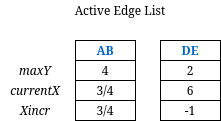
\includegraphics[width=0.4\textwidth]{images/3/3a_ael1.png}
    \caption*{AEL na linha 1.}
\end{figure}
    \item Linha 2: pixels 2-4 (azul).

\begin{figure}[H]
    \centering
    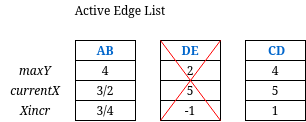
\includegraphics[width=0.4\textwidth]{images/3/3a_ael2.png}
    \caption*{AEL na linha 2.}
\end{figure}
    \item Linha 3: pixels 3-5 (verde).

\begin{figure}[H]
    \centering
    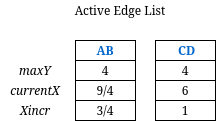
\includegraphics[width=0.4\textwidth]{images/3/3a_ael3.png}
    \caption*{AEL na linha 3.}
\end{figure}
    \item Linha 4: nenhum pixel.

\begin{figure}[H]
    \centering
    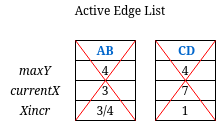
\includegraphics[width=0.4\textwidth]{images/3/3a_ael4.png}
    \caption*{AEL na linha 4.}
\end{figure}
\end{itemize}

Assim, vemos que o polígono A preenchido após a execução do algoritmo na figura \ref{fig:3a_final} abaixo.
\begin{figure}[H]
    \centering
    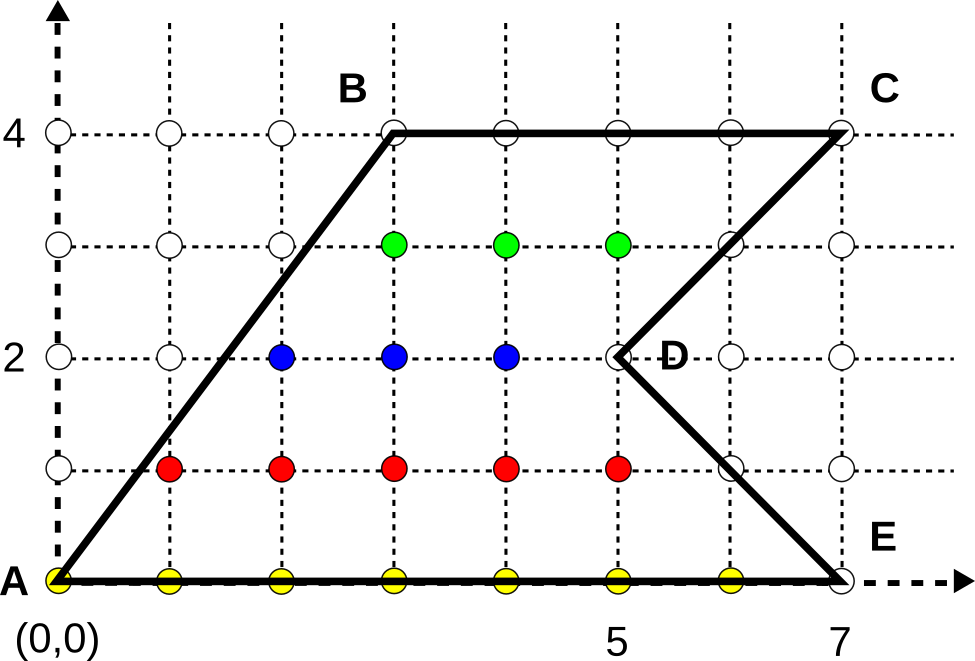
\includegraphics[width=0.4\textwidth]{images/3/3a_final.png}
    \caption{Polígono A preenchido}
    \label{fig:3a_final}
\end{figure}

\textbf{b)}

A AET do polígono B pode ser vista na figura \ref{fig:3b_aet}.

\begin{figure}[H]
    \centering
    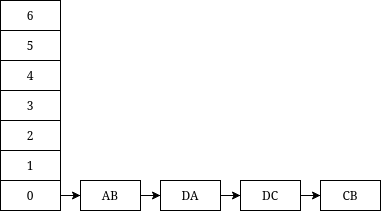
\includegraphics[width=0.5\textwidth]{images/3/3b_aet.png}
    \caption{AET do polígono B}
    \label{fig:3b_aet}
\end{figure}

A cada iteração do algoritmo, se tem uma AEL (\textit{Active Edge List}), a partir da qual são calculados os pixels a serem desenhados. Para cada iteração (ou seja, \textit{scanline}), temos um diagrama da AEL correspondente, e cada iteração desenha pixels na imagem com uma cor específica. No texto, os pixels indicados são os valores em X, como o valor em Y é o mesmo para cada iteração.

\begin{itemize}
    \item Linha 0: nenhum pixel.
\begin{figure}[H]
    \centering
    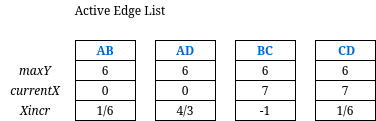
\includegraphics[width=0.5\textwidth]{images/3/3b_ael0.png}
    \caption*{AEL na linha 0.}
\end{figure}
    \item Linha 1: pixels 1 e 6-7 (vermelho).

\begin{figure}[H]
    \centering
    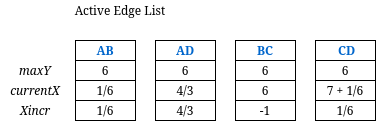
\includegraphics[width=0.5\textwidth]{images/3/3b_ael1.png}
    \caption*{AEL na linha 1.}
\end{figure}
    \item Linha 2: pixels 1-2 e 5-7 (azul).

\begin{figure}[H]
    \centering
    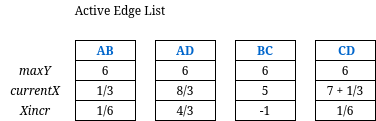
\includegraphics[width=0.5\textwidth]{images/3/3b_ael2.png}
    \caption*{AEL na linha 2.}
\end{figure}
    \item Linha 3: pixels 1-3 e 4-7 (verde).

\begin{figure}[H]
    \centering
    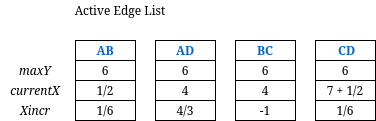
\includegraphics[width=0.5\textwidth]{images/3/3b_ael3.png}
    \caption*{AEL na linha 3.}
\end{figure}
    \item Linha 4: 1-2 e 6-7 (magenta).

\begin{figure}[H]
    \centering
    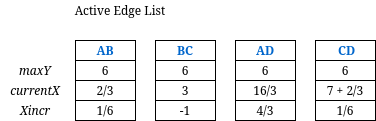
\includegraphics[width=0.5\textwidth]{images/3/3b_ael4.png}
    \caption*{AEL na linha 4.}
\end{figure}
    \item Linha 5: 1 e 7 (ciano).

\begin{figure}[H]
    \centering
    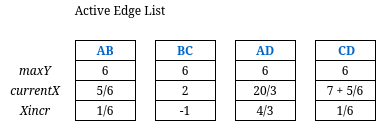
\includegraphics[width=0.5\textwidth]{images/3/3b_ael5.png}
    \caption*{AEL na linha 5.}
\end{figure}
    \item Linha 6: nenhum pixel.

\begin{figure}[H]
    \centering
    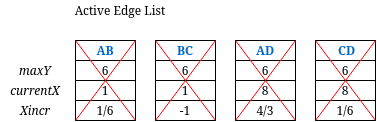
\includegraphics[width=0.5\textwidth]{images/3/3b_ael6.png}
    \caption*{AEL na linha 6.}
\end{figure}
\end{itemize}

Assim, vemos que o polígono A preenchido após a execução do algoritmo na figura \ref{fig:3b_final} abaixo.
\begin{figure}[H]
    \centering
    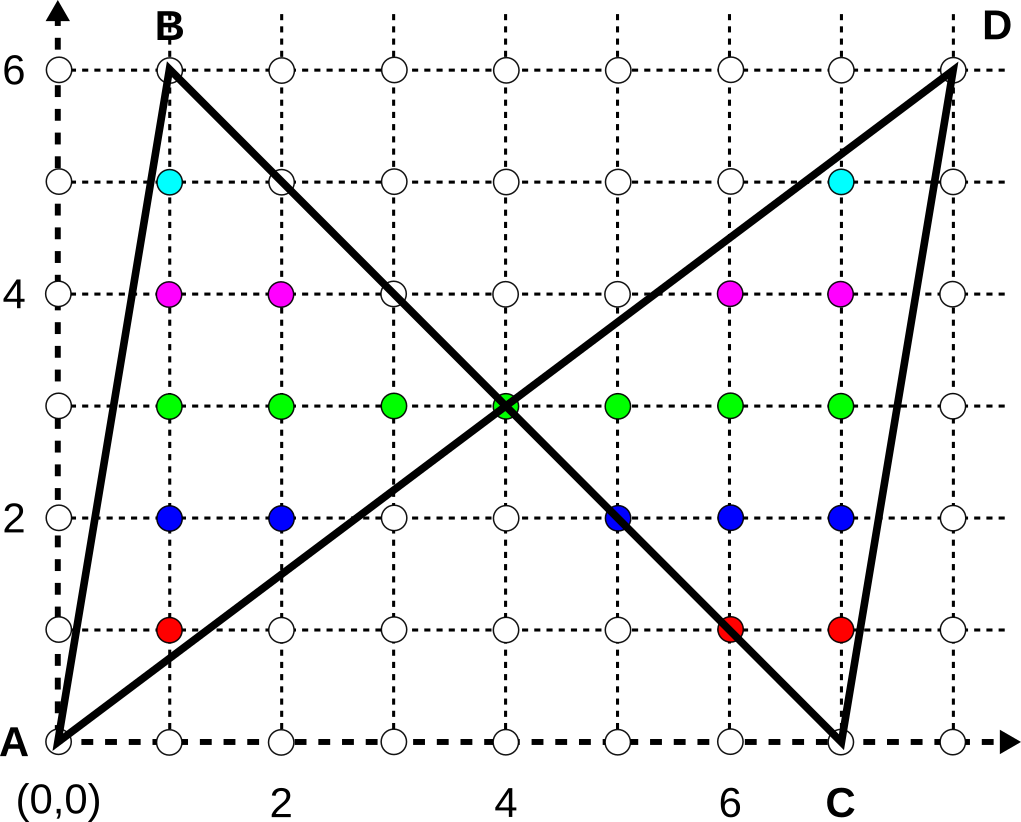
\includegraphics[width=0.4\textwidth]{images/3/3b_final.png}
    \caption{Polígono B preenchido}
    \label{fig:3b_final}
\end{figure}

% %%%%%%%%%%%%%%%%%%%
\section*{Questão 4}
% %%%%%%%%%%%%%%%%%%%
{\bfseries Explique como funcionaria o recorte de linhas de CohenSutherland para o conjunto de linhas abaixo, em relação à janela de recorte dada (indique a sequencia de passos, para cada segmento de reta mostrado).}

\begin{figure}[H]
    \centering
    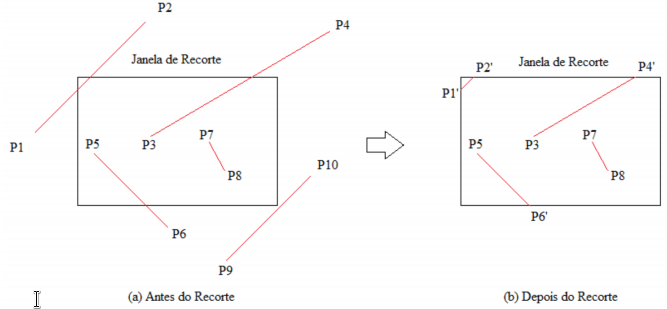
\includegraphics[width=0.9\textwidth]{images/4/4.png}
    \caption{Conjunto de linhas}
    \label{fig:4}
\end{figure}{}

O algoritmo será executado para cada segmento de reta.

No algoritmo de Cohen-Sutherland, cada bit indica se um ponto está dentro ou fora de uma aresta específica da janela. Cada bit indica uma aresta, como pode ser visto na figura \ref{fig:cohen}.

\begin{figure}[H]
    \centering
    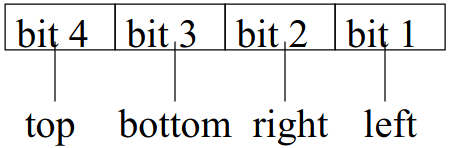
\includegraphics[width=0.3\textwidth]{images/cohen.png}
    \caption{Códigos 2D Cohen-Sutherland}
    \label{fig:cohen}
\end{figure}{}

\begin{itemize}
    \item Segmento P1-P2:
\end{itemize}
$c_0: 0001$ \hspace{1cm} $c_1: 1000$

Ambos vértices estão fora da janela, mas $c_0 \land c_1 = 0$, então esse segmento P1-P2 não é trivialmente rejeitado. Assim, \textit{clipping} é necessário, e faremos a mudança em P1. Logo: P1 se torna P1'.

\begin{figure}[H]
    \centering
    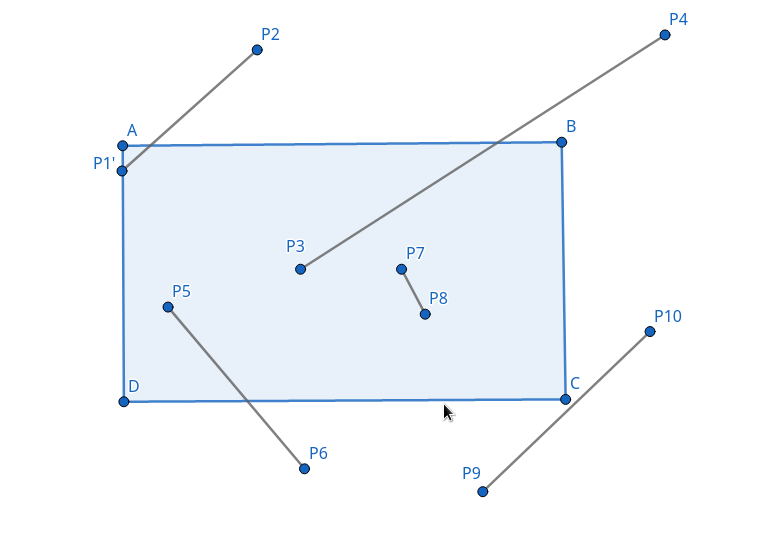
\includegraphics[width=0.5\textwidth]{images/4/4it1.png}
    \caption*{Iteração 1}
\end{figure}

$c_0: 0000$ \hspace{1cm} $c_1: 1000$

P0 está dentro da janela, e P1 está fora da janela, então o segmento P1'-P2 não é trivialmente aceito ou rejeitado. Assim, \textit{clipping} é necessário, modificando P2. Logo: P2 se torna P2'.

\begin{figure}[H]
    \centering
    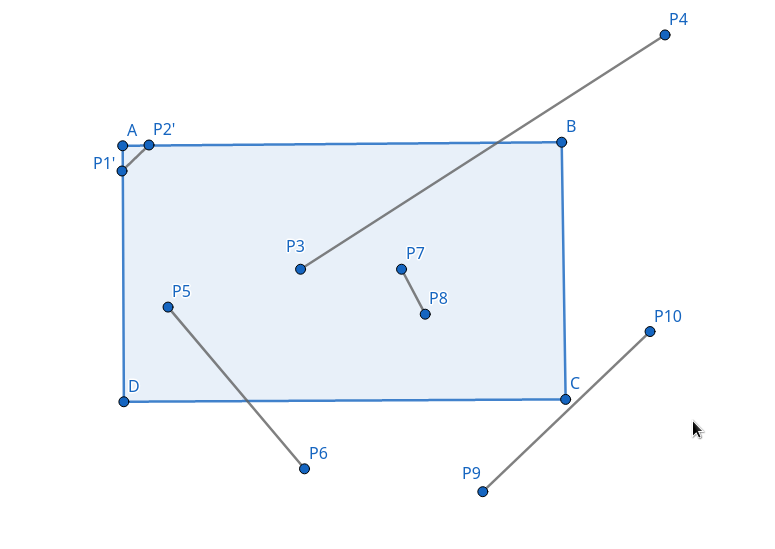
\includegraphics[width=0.5\textwidth]{images/4/4it2.png}
    \caption*{Iteração 2}
\end{figure}

$c_0: 0000$ \hspace{1cm} $c_1: 0000$

Ambos vértices estão dentro da janela, com código zero então $c_0 \lor c_1 = 0$. Portanto, o segmento P1'-P2' é aceito trivialmente.

\begin{itemize}
    \item Segmento P3-P4:
\end{itemize}
$c_0: 0000$ \hspace{1cm} $c_1: 1010$

P3 está dentro da janela, e P4 está fora da janela, então o segmento P3-P4 não é trivialmente aceito ou rejeitado. Assim, \textit{clipping} é necessário, modificando P4. Logo: P4 se torna $P4_b$.

\begin{figure}[H]
    \centering
    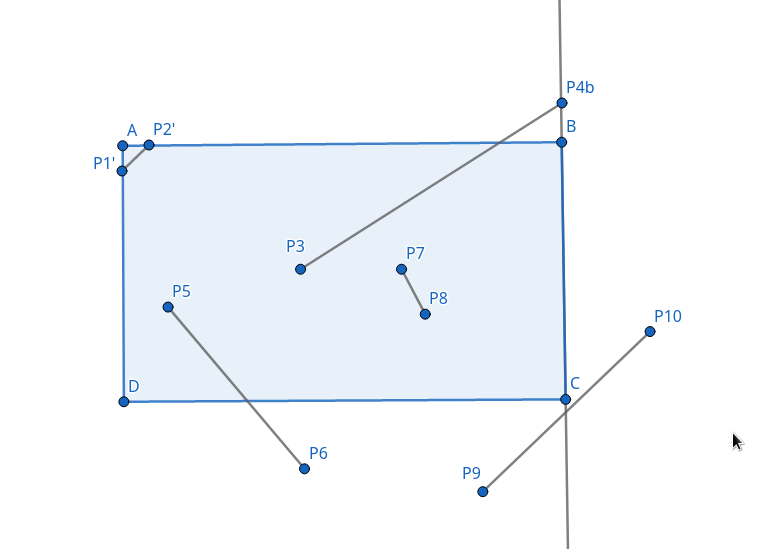
\includegraphics[width=0.5\textwidth]{images/4/4it3.png}
    \caption*{Iteração 3}
\end{figure}

$c_0: 0000$ \hspace{1cm} $c_1: 1000$

P3 está dentro da janela, e $P4_b$ está fora da janela, então o segmento P3-$P4_b$ não é trivialmente aceito ou rejeitado. Assim, \textit{clipping} é necessário, modificando $P4_b$. Logo: $P4_b$ se torna P4'.

\begin{figure}[H]
    \centering
    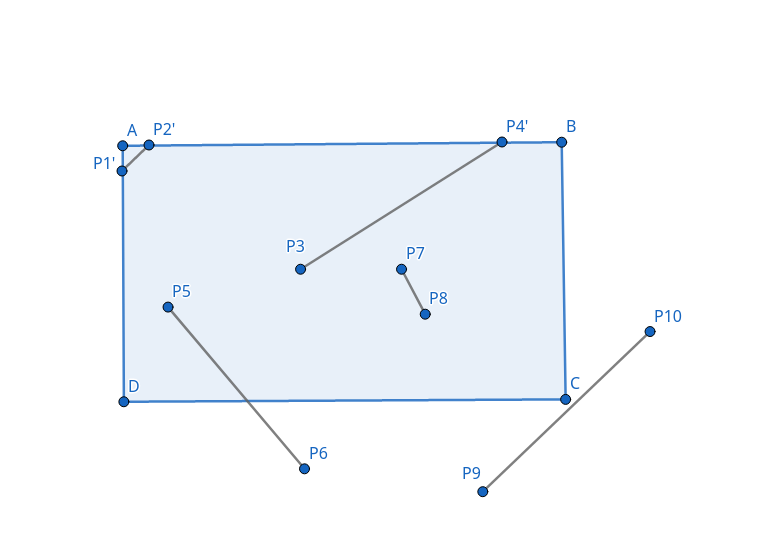
\includegraphics[width=0.5\textwidth]{images/4/4it4.png}
    \caption*{Iteração 4}
\end{figure}

$c_0: 0000$ \hspace{1cm} $c_1: 0000$

Ambos vértices estão dentro da janela, com código zero então $c_0 \lor c_1 = 0$. Portanto, o segmento P3-P4' é aceito trivialmente.

\begin{itemize}
    \item Segmento P5-P6:
\end{itemize}
$c_0: 0000$ \hspace{1cm} $c_1: 0100$

P5 está dentro da janela, e P6 está fora da janela, então o segmento P5-P6 não é trivialmente aceito ou rejeitado. Assim, \textit{clipping} é necessário, modificando P6. Logo: P6 se torna P6'.

\begin{figure}[H]
    \centering
    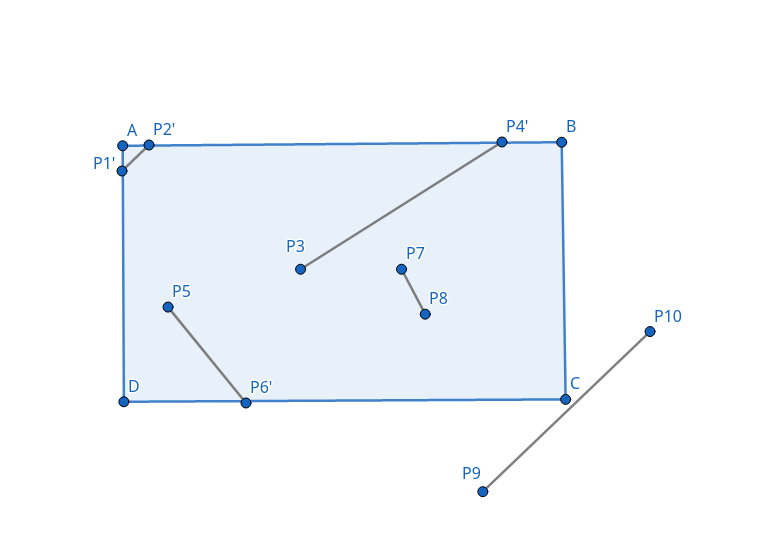
\includegraphics[width=0.5\textwidth]{images/4/4it5.png}
    \caption*{Iteração 5}
\end{figure}

$c_0: 0000$ \hspace{1cm} $c_1: 0000$

Ambos vértices estão dentro da janela, com código zero então $c_0 \lor c_1 = 0$. Portanto, o segmento P5-P6' é aceito trivialmente.

\begin{itemize}
    \item Segmento P7-P8:
\end{itemize}
$c_0: 0000$ \hspace{1cm} $c_1: 0000$

Ambos vértices estão dentro da janela, com código zero então $c_0 \lor c_1 = 0$. Portanto, o segmento P7-P8 é aceito trivialmente.

\begin{itemize}
    \item Segmento P9-P10:
\end{itemize}
$c_0: 0100$ \hspace{1cm} $c_1: 0010$

Ambos vértices estão fora da janela, mas $c_0 \land c_1 = 0$, então esse segmento P9-P10 não é trivialmente rejeitado. Assim, \textit{clipping} é necessário, e faremos a mudança em P9. Logo: P9 se torna P9'.

\begin{figure}[H]
    \centering
    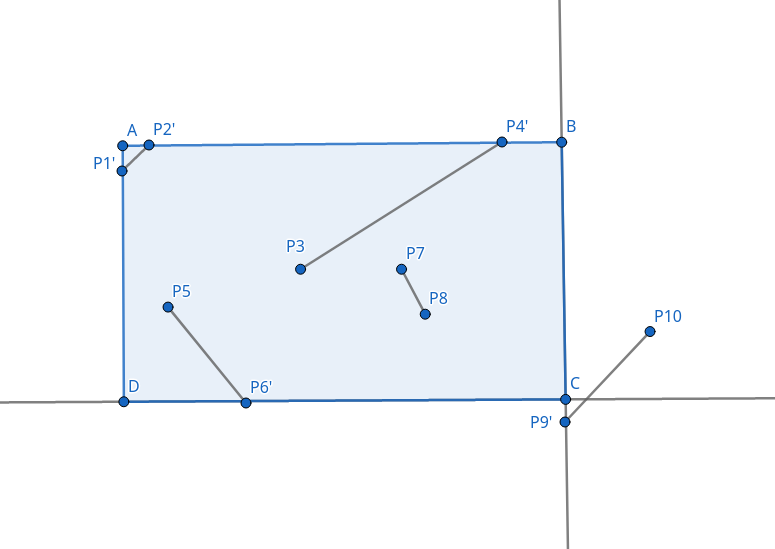
\includegraphics[width=0.5\textwidth]{images/4/4it6.png}
    \caption*{Iteração 6}
\end{figure}\textbf{}

$c_0: 0110$ \hspace{1cm} $c_1: 0010$

Ambos vértices estão fora da janela, e $c_0 \land c_1 \ne 0$, então segmento P9'-P10 é trivialmente rejeitado.

\begin{figure}[H]
    \centering
    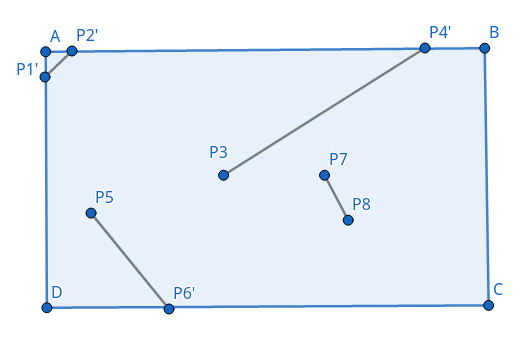
\includegraphics[width=0.5\textwidth]{images/4/4final.png}
    \caption*{Resultado Final}
\end{figure}

% %%%%%%%%%%%%%%%%%%%
\section*{Questão 5}
% %%%%%%%%%%%%%%%%%%%
{\bfseries Explique como funcionaria o recorte de polígonos de SutherlandHodgman para o polígono abaixo, em relação à janela de recorte dada (indique a sequência de passos que seriam executados pelo algoritmo).}

\begin{figure}[H]
    \centering
    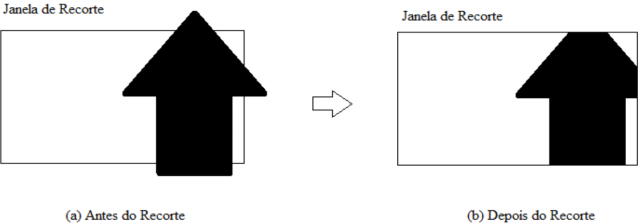
\includegraphics[width=0.9\textwidth]{images/5/5.png}
    \caption{Polígono}
    \label{fig:5}
\end{figure}{}
Na execução do algoritmo, os lados testados são, em ordem, o esquerdo, o direito, o superior e enfim o inferior (left, right, up, bottom, in order).

\begin{figure}[H]
    \centering
    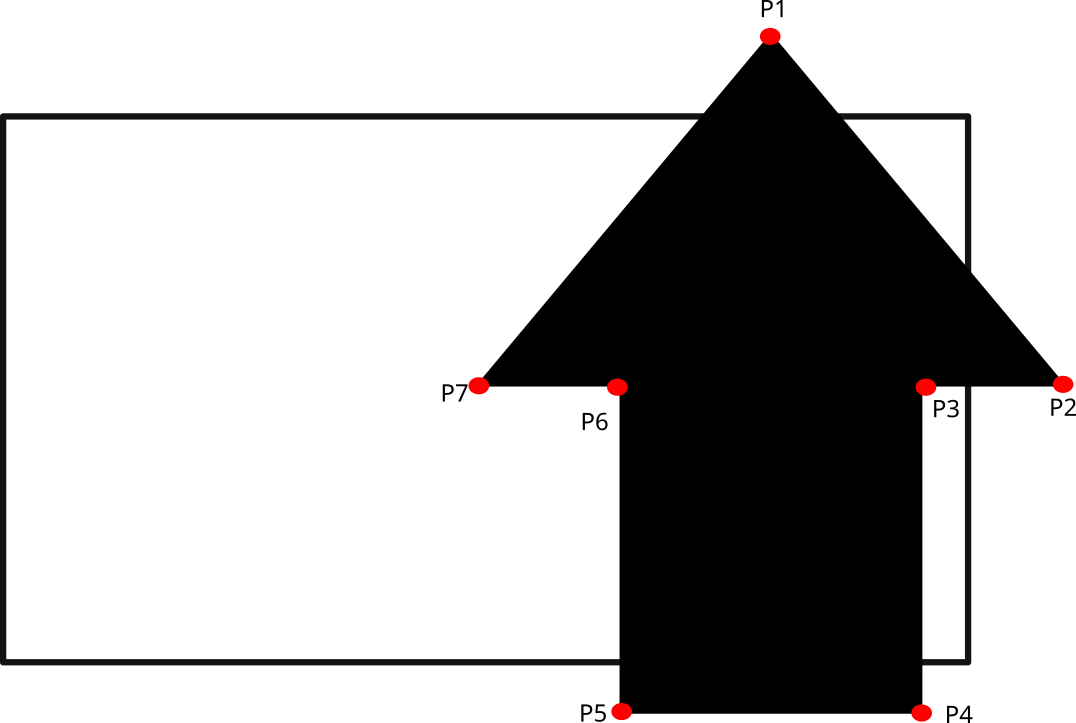
\includegraphics[width=0.5\textwidth]{images/5/5init.png}
    \caption*{Imagem inicial, com pontos destacados.}
\end{figure}{}

\begin{itemize}
    \item Lado esquerdo.
\end{itemize}{}
Analisando o lado esquerdo, a saída é igual à entrada, pois não há interseção do polígono naquele lado. Podemos pular a execução nesse lado.

$L: .P7P6P5P4P3P2P1 \xrightarrow{} R: \xrightarrow{} U: \xrightarrow{} B:$

$L: \xrightarrow{} R: .P1P7P6P5P4P3P2 \xrightarrow{} U: \xrightarrow{} B:$

\begin{figure}[H]
    \centering
    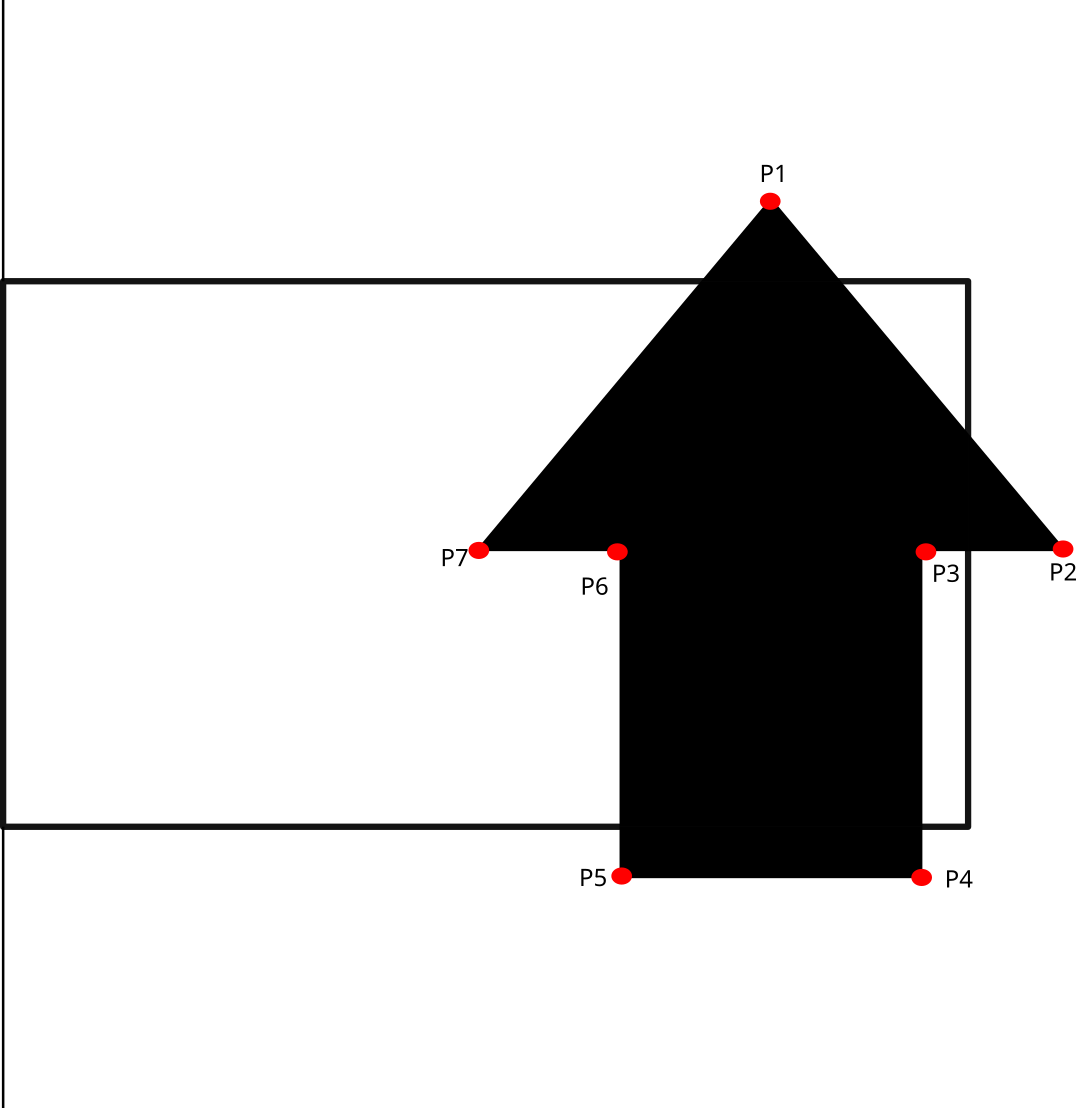
\includegraphics[width=0.5\textwidth]{images/5/5it1.png}
    \caption*{Imagem após iterações do lado esquerdo.}
\end{figure}{}

\begin{itemize}
    \item Lado direito.
\end{itemize}{}

$L: \xrightarrow{} R: .P1P7P6P5P4P3P2 \xrightarrow{} U: \xrightarrow{} B:$

$L: \xrightarrow{} R: .P1P7P6P5P4P3 \xrightarrow{} U: P3a \xrightarrow{} B:$

\begin{figure}[H]
    \centering
    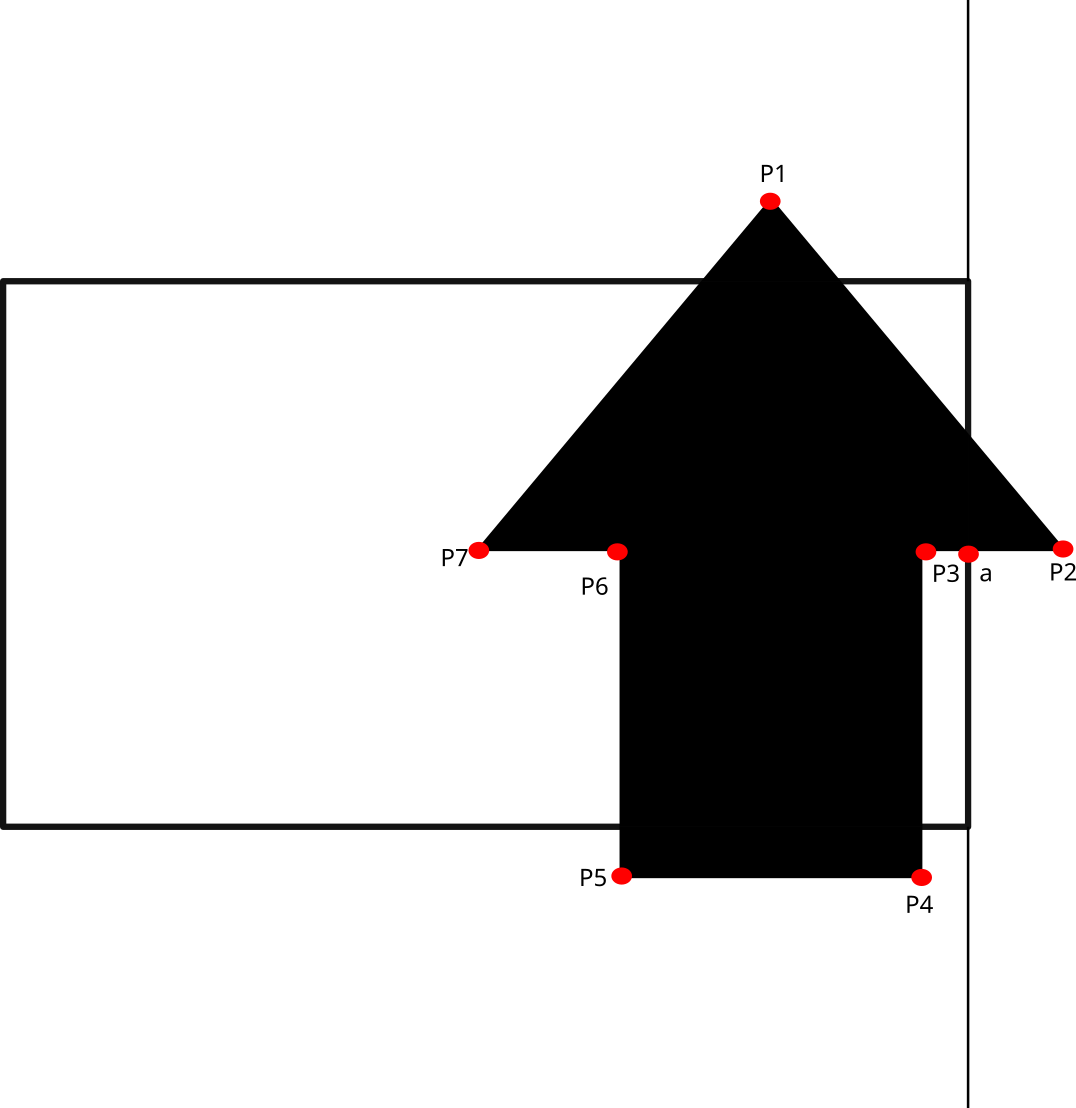
\includegraphics[width=0.5\textwidth]{images/5/5it2.png}
    \caption*{Imagem após primeira iteração do lado direito.}
\end{figure}{}

$L: \xrightarrow{} R: .P1P7P6P5P4 \xrightarrow{} U: P4P3a \xrightarrow{} B:$

$L: \xrightarrow{} R: .P1P7P6P5 \xrightarrow{} U: P5P4P3a \xrightarrow{} B:$

$L: \xrightarrow{} R: .P1P7P6 \xrightarrow{} U: P6P5P4P3a \xrightarrow{} B:$

$L: \xrightarrow{} R: .P1P7 \xrightarrow{} U: P7P6P5P4P3a \xrightarrow{} B:$

$L: \xrightarrow{} R: .P1 \xrightarrow{} U: P1P7P6P5P4P3a \xrightarrow{} B:$

$L: \xrightarrow{} R: . \xrightarrow{} U: bP1P7P6P5P4P3a \xrightarrow{} B:$

\begin{figure}[H]
    \centering
    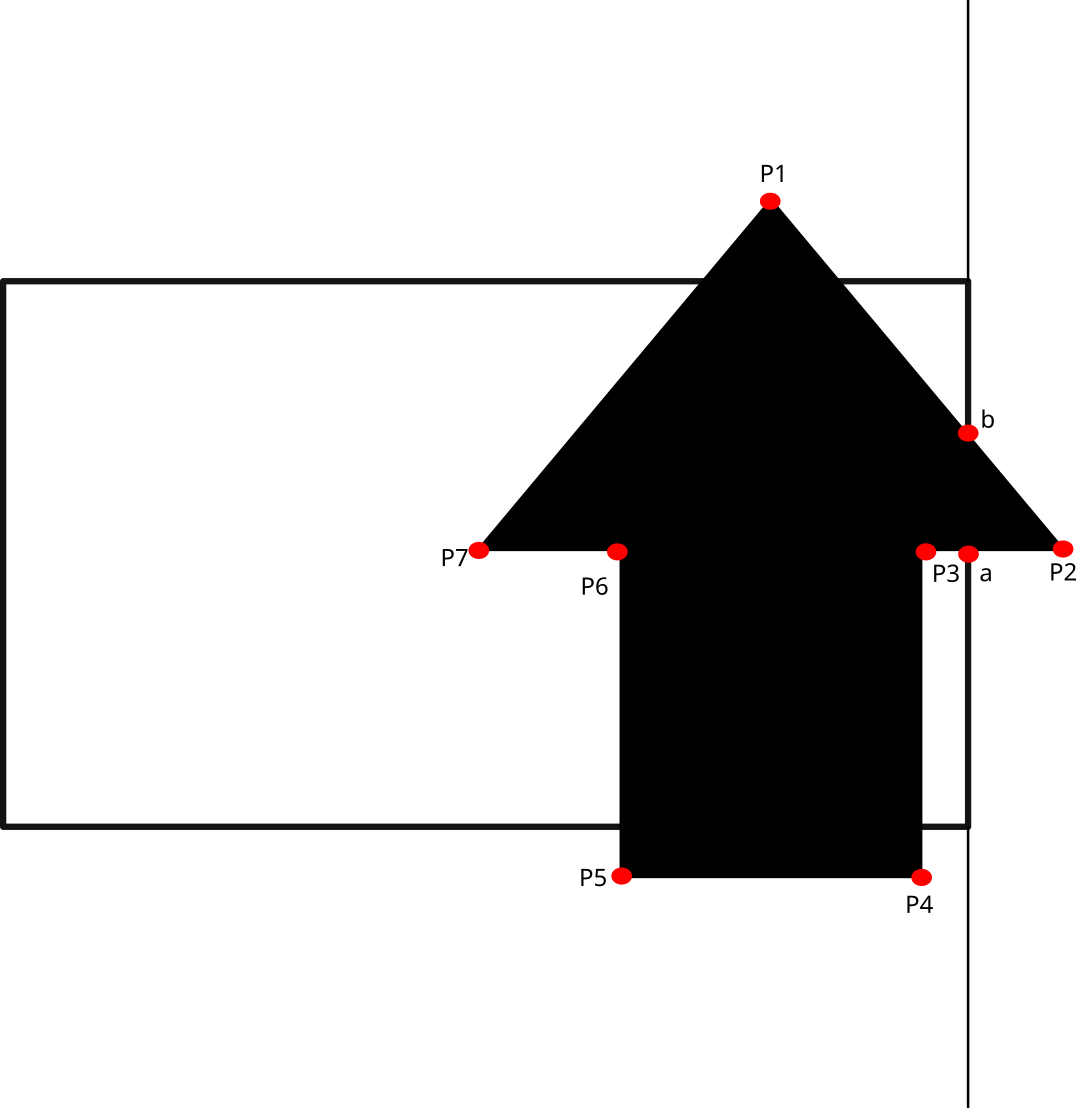
\includegraphics[width=0.5\textwidth]{images/5/5it3.png}
    \caption*{Imagem após iterações do lado direito.}
\end{figure}{}

$L: \xrightarrow{} R: \xrightarrow{} U: .bP1P7P6P5P4P3a \xrightarrow{} B:$

\begin{itemize}
    \item Lado superior.
\end{itemize}

$L: \xrightarrow{} R: \xrightarrow{} U: .bP1P7P6P5P4P3a \xrightarrow{} B:$

$L: \xrightarrow{} R: \xrightarrow{} U: .bP1P7P6P5P4P3 \xrightarrow{} B: P3$

$L: \xrightarrow{} R: \xrightarrow{} U: .bP1P7P6P5P4 \xrightarrow{} B: P4P3$

$L: \xrightarrow{} R: \xrightarrow{} U: .bP1P7P6P5 \xrightarrow{} B: P5P4P3$

$L: \xrightarrow{} R: \xrightarrow{} U: .bP1P7P6 \xrightarrow{} B: P6P5P4P3$

$L: \xrightarrow{} R: \xrightarrow{} U: .bP1P7 \xrightarrow{} B: P7P6P5P4P3$

$L: \xrightarrow{} R: \xrightarrow{} U: .bP1 \xrightarrow{} B: cP7P6P5P4P3$

\begin{figure}[H]
    \centering
    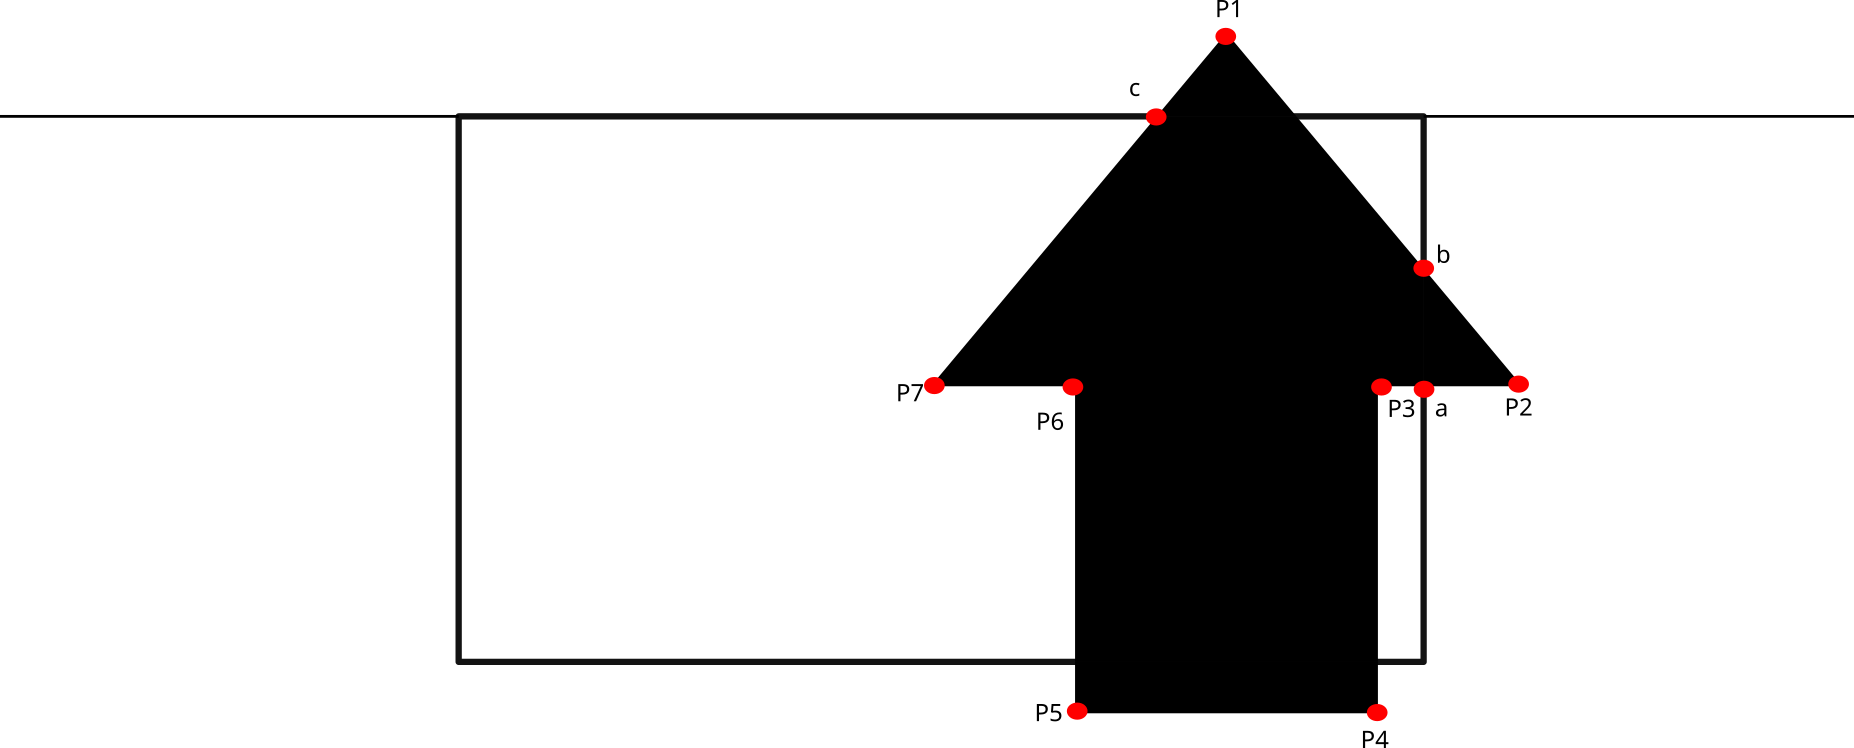
\includegraphics[width=0.7\textwidth]{images/5/5it4.png}
    \caption*{Imagem após primeira interseção do lado superior.}
\end{figure}{}

$L: \xrightarrow{} R: \xrightarrow{} U: .b \xrightarrow{} B: bdcP7P6P5P4P3$

\begin{figure}[H]
    \centering
    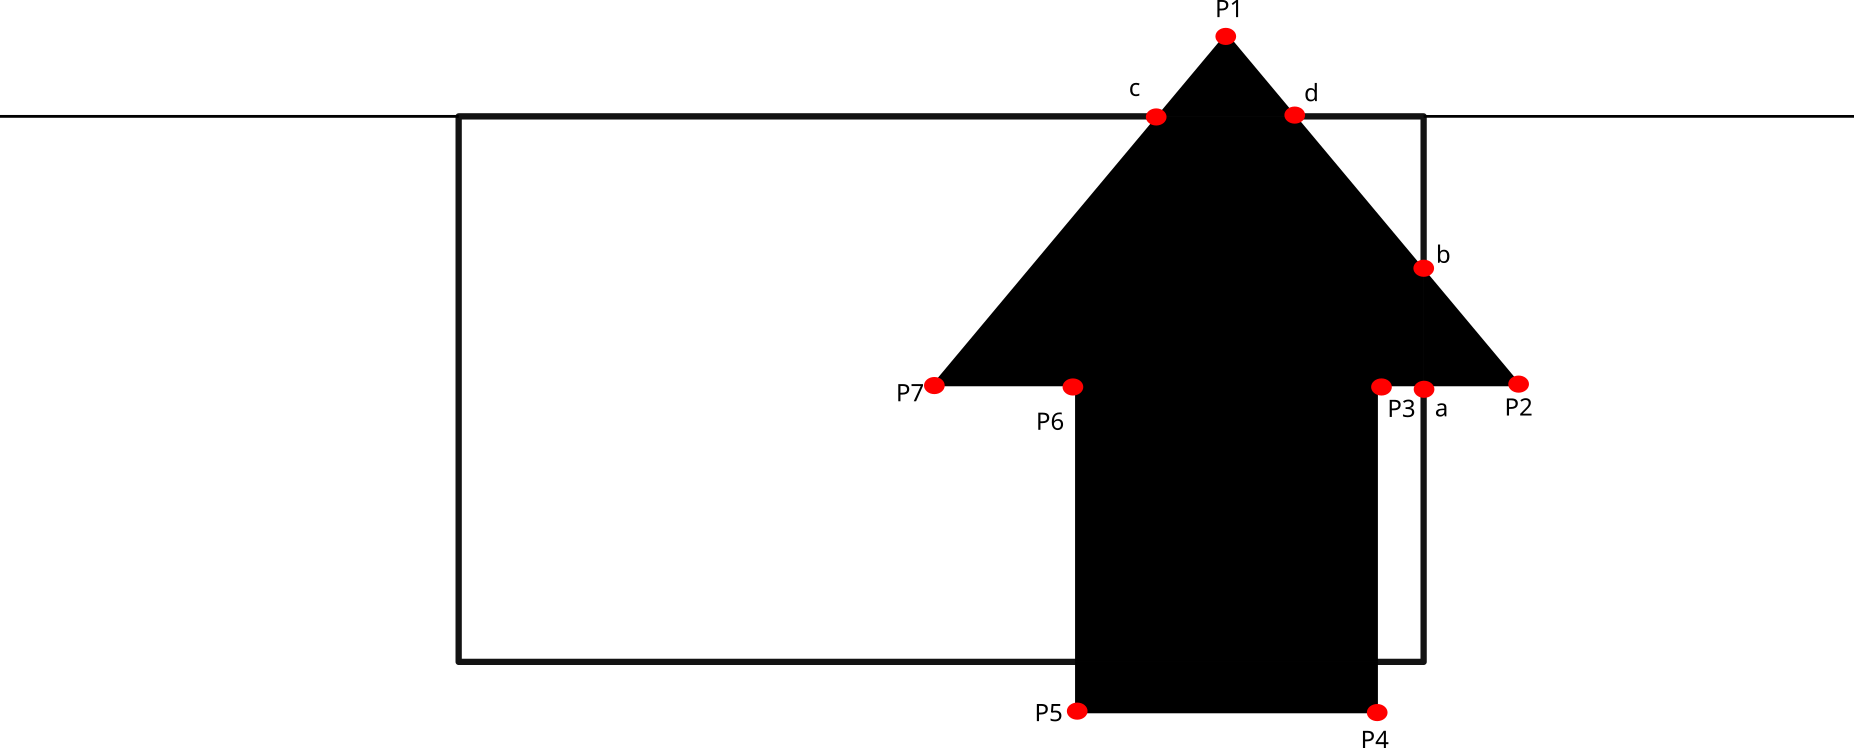
\includegraphics[width=0.7\textwidth]{images/5/5it5.png}
    \caption*{Imagem após segunda interseção do lado superior.}
\end{figure}{}

$L: \xrightarrow{} R: \xrightarrow{} U: . \xrightarrow{} B: abdcP7P6P5P4P3$

$L: \xrightarrow{} R: \xrightarrow{} U: \xrightarrow{} B: .abdcP7P6P5P4P3$

\begin{itemize}
    \item Lado inferior.
\end{itemize}

$L: \xrightarrow{} R: \xrightarrow{} U: \xrightarrow{} B: .abdcP7P6P5P4P3 \xrightarrow{} $

$L: \xrightarrow{} R: \xrightarrow{} U: \xrightarrow{} B: .abdcP7P6P5P4 \xrightarrow{} e$

\begin{figure}[H]
    \centering
    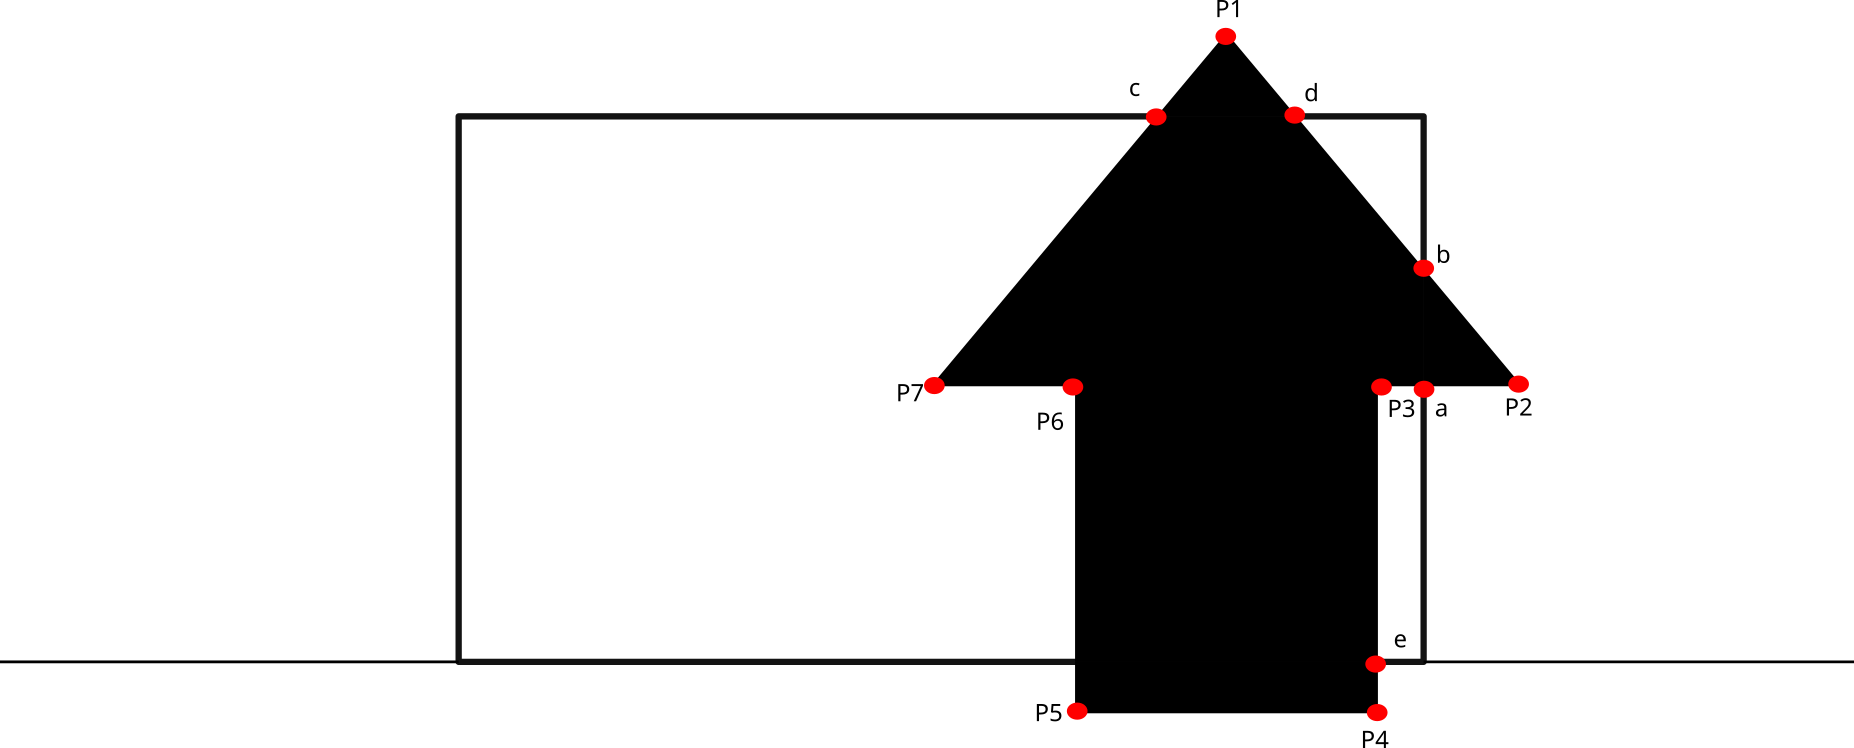
\includegraphics[width=0.7\textwidth]{images/5/5it6.png}
    \caption*{Imagem após primeira interseção do lado inferior.}
\end{figure}{}

$L: \xrightarrow{} R: \xrightarrow{} U: \xrightarrow{} B: .abdcP7P6P5 \xrightarrow{} e$

$L: \xrightarrow{} R: \xrightarrow{} U: \xrightarrow{} B: .abdcP7P6 \xrightarrow{} P6fe$

\begin{figure}[H]
    \centering
    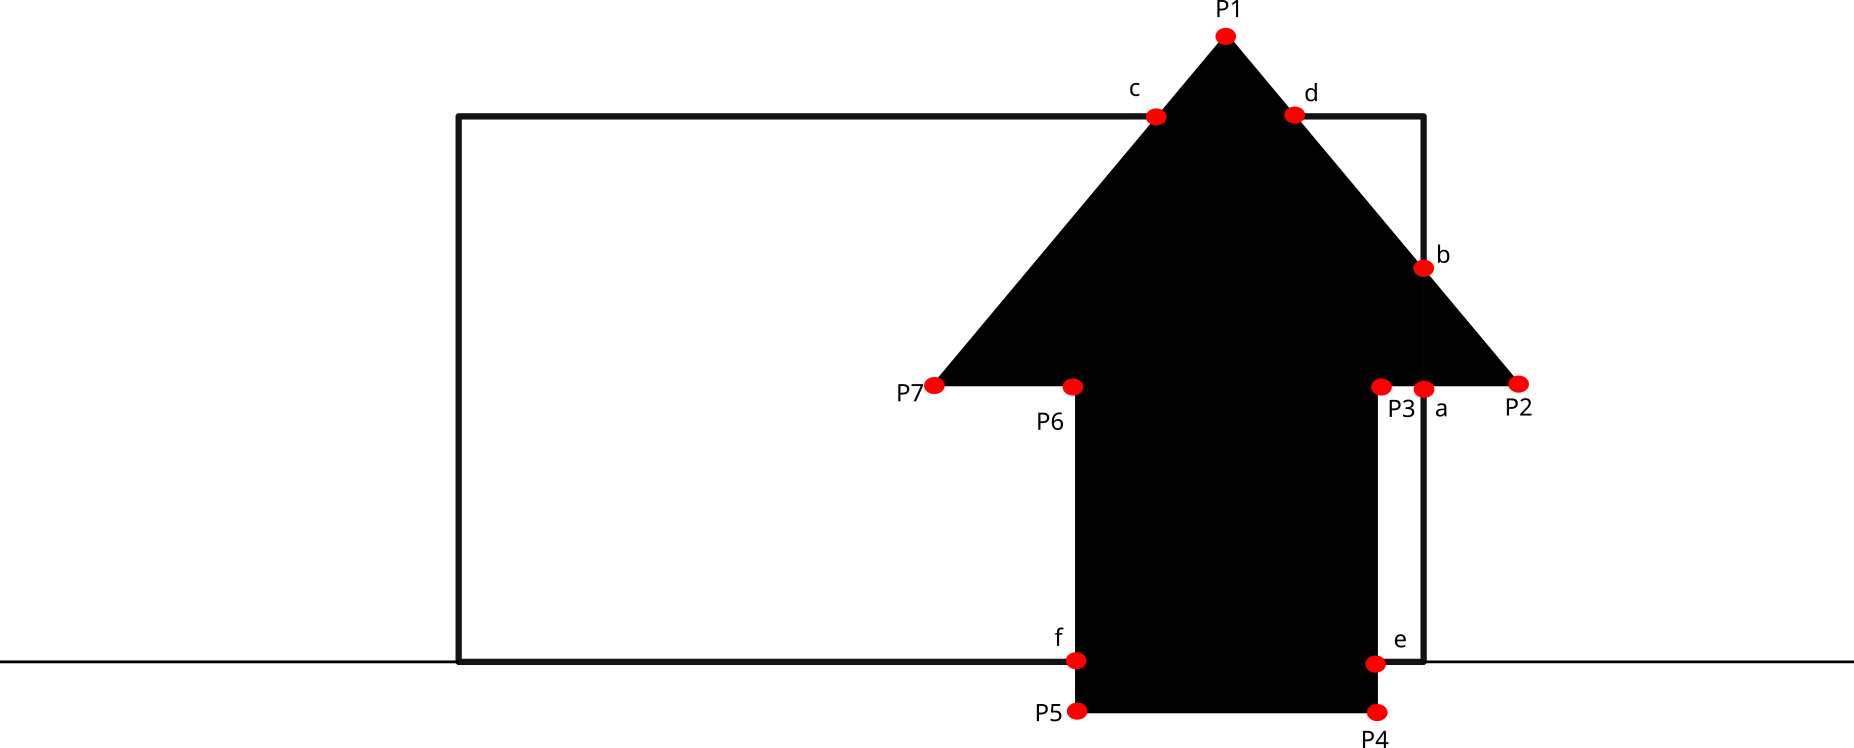
\includegraphics[width=0.7\textwidth]{images/5/5it7.png}
    \caption*{Imagem após segunda interseção do lado inferior.}
\end{figure}{}

$L: \xrightarrow{} R: \xrightarrow{} U: \xrightarrow{} B: .abdcP7 \xrightarrow{} P7P6fe$

$L: \xrightarrow{} R: \xrightarrow{} U: \xrightarrow{} B: .abdc \xrightarrow{} cP7P6fe$

$L: \xrightarrow{} R: \xrightarrow{} U: \xrightarrow{} B: .abd \xrightarrow{} dcP7P6fe$

$L: \xrightarrow{} R: \xrightarrow{} U: \xrightarrow{} B: .ab \xrightarrow{} bdcP7P6fe$

$L: \xrightarrow{} R: \xrightarrow{} U: \xrightarrow{} B: .a \xrightarrow{} abdcP7P6fe$

$L: \xrightarrow{} R: \xrightarrow{} U: \xrightarrow{} B: . \xrightarrow{} P3abdcP7P6fe$

$L: \xrightarrow{} R: \xrightarrow{} U: \xrightarrow{} B: \xrightarrow{} .P3abdcP7P6fe$

\begin{figure}[H]
    \centering
    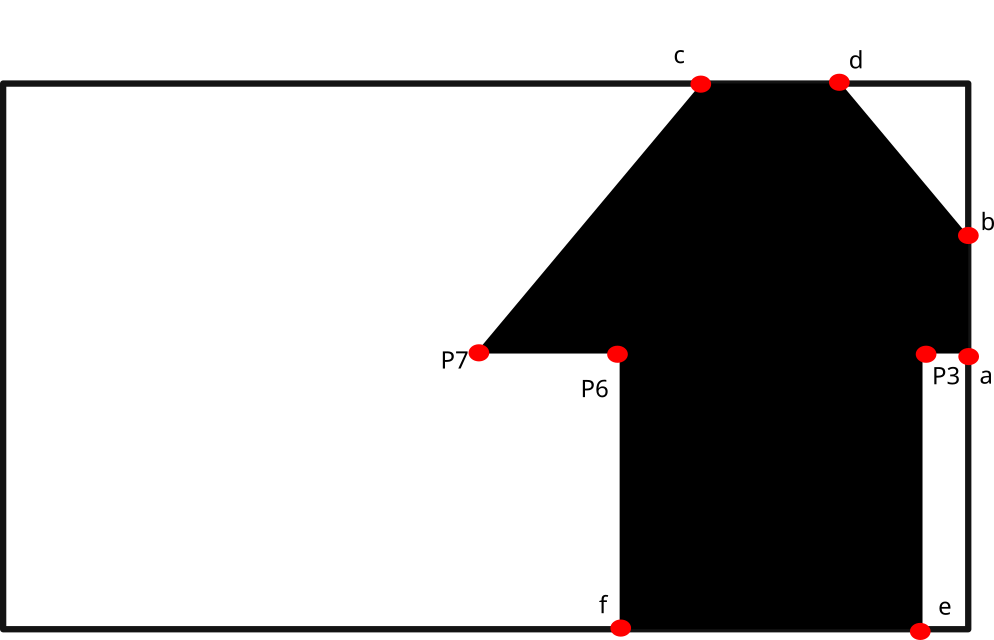
\includegraphics[width=0.5\textwidth]{images/5/5final.png}
    \caption*{Imagem final após \textit{clipping}.}
\end{figure}{}

Temos assim que a sequência final de vértices do polígono resultante é "e,f,P6,P7,c,d,b,a,P3".

% %%%%%%%%%%%%%%%%%%%
\section*{Questão 6}
% %%%%%%%%%%%%%%%%%%%
{\bfseries Indique verdadeiro ou falso e justifique a resposta:}

\begin{enumerate}[label=\alph*)]
    \item A composição de duas translações comuta. (V)
\end{enumerate}

Uma translação pelo vetor $(x_1, y_1)$ e outra pelo vetor $(x_2, y_2)$ é o mesmo que uma translação pelo vetor $(x_1+x_2, y_1+y_2)$. Isso pode ser visto tanto pela translação utilizando soma quanto a em coordenadas homogêneas. Como a operação de soma é comutativa, a translação também é. Por isso a afirmação é verdadeira.

\begin{enumerate}[label=\alph*), resume]
    \item Toda transformação afim é uma transformação rígida. (F)
\end{enumerate}

A afirmação é falsa pois inverte as posições de ambos tipos de transformação na hierarquia. Toda transformação rígida é uma transformação afim, porém as transformações rígidas são um subconjunto incompleto das afins, não englobando escala, reflexão, cisalhamento e outras transformações afins. 

\begin{enumerate}[label=\alph*), resume]
    \item A imagem do ponto (4, -3) sob uma reflexão no eixo x é (-4, -3). (F)
\end{enumerate}

A afirmação é falsa pois uma reflexão no eixo x implica que a coordenada do ponto em x se mantém, sendo refletida a coordenada em y para o outro lado do eixo x, ou seja, $y_f = -y_i$, ao contrário da afirmação, que inverte a coordenada em x. A afirmação mostra uma reflexão no eixo y. Uma reflexão no eixo x seria (4, 3).

\begin{enumerate}[label=\alph*), resume]
    \item A imagem do ponto (-5, 4) sob uma reflexão através do eixo y é (5, 4). (V)
\end{enumerate}

A afirmação é verdadeira pois uma reflexão no eixo y implica que a coordenada do ponto em y se mantém, sendo refletida a coordenada em x para o outro lado do eixo y, ou seja, $x_f = -x_i$, assim como afirmado.

% %%%%%%%%%%%%%%%%%%%
\section*{Questão 7}
% %%%%%%%%%%%%%%%%%%%
{\bfseries Dadas as seguintes figuras, desenhe a imagem do resultado da figura após a transformação e defina o tipo de transformação em cada caso.}

\begin{enumerate}[label=\alph*)]
    \item (x,y) $\xrightarrow{}$ (x,-y). 
\end{enumerate}

\begin{figure}[H]
    \centering
    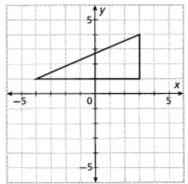
\includegraphics{images/7a.png}
    \caption{7A}
    \label{fig:7a}
\end{figure}{}

A transformação da figura \ref{fig:7a} é uma \textbf{reflexão através do eixo x.}

As coordenadas da imagem são (-4,1), (3,1) e (3,4), então após a reflexão o resultado é (-4,-1), (3,-1), (3,-4). O resultado está na figura \ref{fig:7a_resp} abaixo:

\begin{figure}[H]
    \centering
    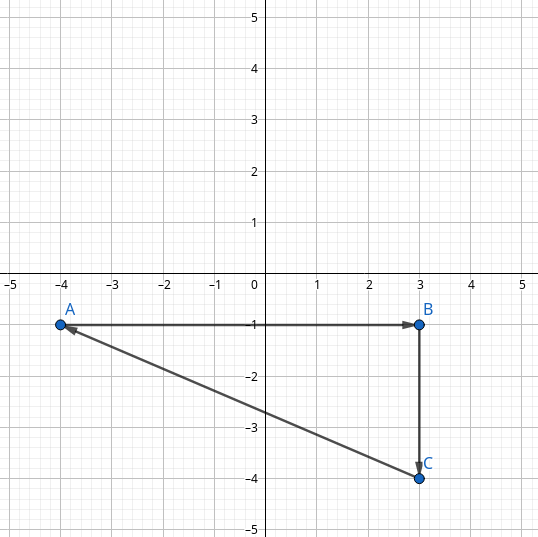
\includegraphics[width=0.5\textwidth]{images/7a_resp.png}
    \caption{Resultado do item 7a.}
    \label{fig:7a_resp}
\end{figure}{}


\begin{enumerate}[label=\alph*), resume]
    \item (x,y) $\xrightarrow{}$ (x,3y). 
\end{enumerate}

\begin{figure}[H]
    \centering
    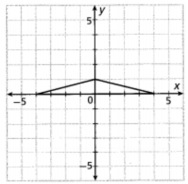
\includegraphics{images/7b.png}
    \caption{7B}
    \label{fig:7b}
\end{figure}{}

A transformação da figura \ref{fig:7b} é uma \textbf{escala com fator 3 em y e fator 1 em x}. 

As coordenadas da imagem são (0,1), (-4,0) e (4,0), então após a escala o resultado é (0,3), (-4,0), (4,0). O resultado está na figura \ref{fig:7b_resp} abaixo:

\begin{figure}[H]
    \centering
    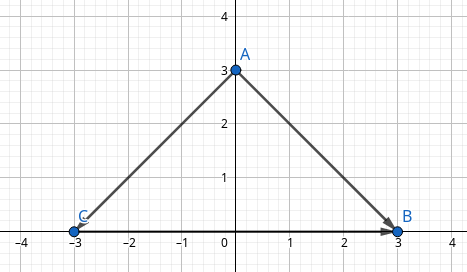
\includegraphics[width=0.5\textwidth]{images/7b_resp.png}
    \caption{Resultado do item 7b.}
    \label{fig:7b_resp}
\end{figure}{}

\begin{enumerate}[label=\alph*), resume]
    \item (x,y) $\xrightarrow{}$ (x-4,y-4). 
\end{enumerate}

\begin{figure}[H]
    \centering
    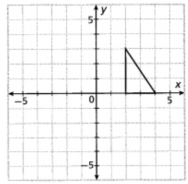
\includegraphics{images/7c.png}
    \caption{7C}
    \label{fig:7c}
\end{figure}{}

A transformação da figura \ref{fig:7c} é uma \textbf{translação com offset em x igual a -4 e offset em y igual a -4}. 

As coordenadas da imagem são (2,3), (2,0) e (4,0), então após a translação o resultado é (-2,-1), (-2,-4), (0,-4). O resultado está na figura \ref{fig:7c_resp} abaixo:

\begin{figure}[H]
    \centering
    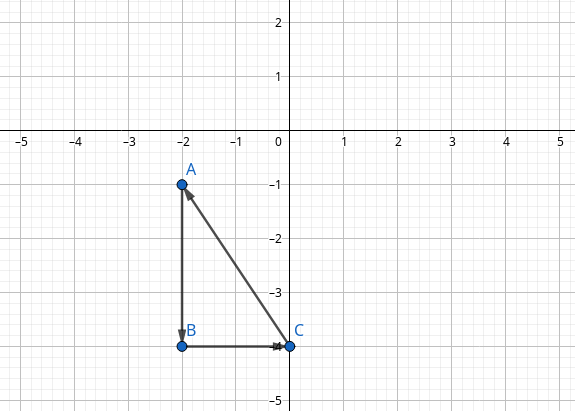
\includegraphics[width=0.6\textwidth]{images/7c_resp.png}
    \caption{Resultado do item 7c.}
    \label{fig:7c_resp}
\end{figure}{}

% %%%%%%%%%%%%%%%%%%%
\section*{Questão 8}
% %%%%%%%%%%%%%%%%%%%
{\bfseries Matriz de transformação:}

\begin{enumerate}[label=\alph*)]
    \item Construa a equação para a matriz de transformação que faça a translação T(3,2) e a rotação R(30\degree), nesta ordem, para o objeto abaixo. Execute a operação para cada um dos pontos e faça o gráfico da nova posição do objeto.
\end{enumerate}

\begin{figure}[H]
    \centering
    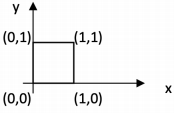
\includegraphics{images/8a.png}
    \caption{8A}
    \label{fig:8a}
\end{figure}

Queremos uma rotação em 30\degree. Assim, precisamos dos valores de seno e cosseno desse valor.
$\sin{30\degree} = \frac{1}{2}$ \hspace{2em} $\cos{30\degree} = \frac{\sqrt{3}}{2}$

Com esses valores, podemos construir a matriz de rotação em 30\degree. Para realizar ambas transformações, precisamos realizar uma operação de composição. Então, $A$ sendo a transformação desejada, $R$ sendo a rotação e $T$ a translação, temos que:
\begin{gather*}
    \begin{bmatrix}
    x' \\
    y' \\
    1
    \end{bmatrix}
    = R \cdot T \cdot
    \begin{bmatrix}
    x \\
    y \\
    1
    \end{bmatrix} \\
    P' = A \cdot P \\
    A = R \cdot T
\end{gather*}

Vemos então que a composição é feita de, na ordem, $R\cdot T$. $R$ e $T$ são dados por:

\begin{gather*}
    \renewcommand\arraystretch{2}
    R=
    \begin{bmatrix}
    \cos{30\degree} & -\sin{30\degree} & 0 \\
    \sin{30\degree} & \cos{30\degree} & 0 \\
    0 & 0 & 1
    \end{bmatrix} 
    =
    \begin{bmatrix}
    \frac{\sqrt{3}}{2} & -\frac{1}{2} & 0 \\
    \frac{1}{2} & \frac{\sqrt{3}}{2} & 0 \\
    0 & 0 & 1
    \end{bmatrix}\\
    T = 
    \begin{bmatrix}
    1 & 0 & T_x \\
    0 & 1 & T_y \\
    0 & 0 & 1
    \end{bmatrix}
    =
    \begin{bmatrix}
    1 & 0 & 3 \\
    0 & 1 & 2 \\
    0 & 0 & 1
    \end{bmatrix}    
\end{gather*}

Assim, a composição fica:
\begin{equation*}
    \renewcommand\arraystretch{2}
    A = 
    \begin{bmatrix}
    \frac{\sqrt{3}}{2} & -\frac{1}{2} & 0 \\
    \frac{1}{2} & \frac{\sqrt{3}}{2} & 0 \\
    0 & 0 & 1
    \end{bmatrix}
    \cdot
    \begin{bmatrix}
    1 & 0 & 3 \\
    0 & 1 & 2 \\
    0 & 0 & 1
    \end{bmatrix}
    =
    \begin{bmatrix}
    \frac{\sqrt{3}}{2} & -\frac{1}{2} & \frac{3\sqrt{3}-2}{2} \\
    \frac{1}{2} & \frac{\sqrt{3}}{2} & \frac{3}{2} + \sqrt{3} \\
    0 & 0 & 1
    \end{bmatrix}
\end{equation*}

As coordenadas do objeto da figura \ref{fig:8a} são (0,0), (0,1), (1,0), (1,1). Após a transformação, as coordenadas finais são (1.6, 3.2), (1.1, 4.1), (2.5, 3.7), (2.0, 4.6), arredondando para 1 casa decimal. O resultado pode ser visto na figura \ref{fig:8a_resp} abaixo:

\begin{figure}[H]
    \centering
    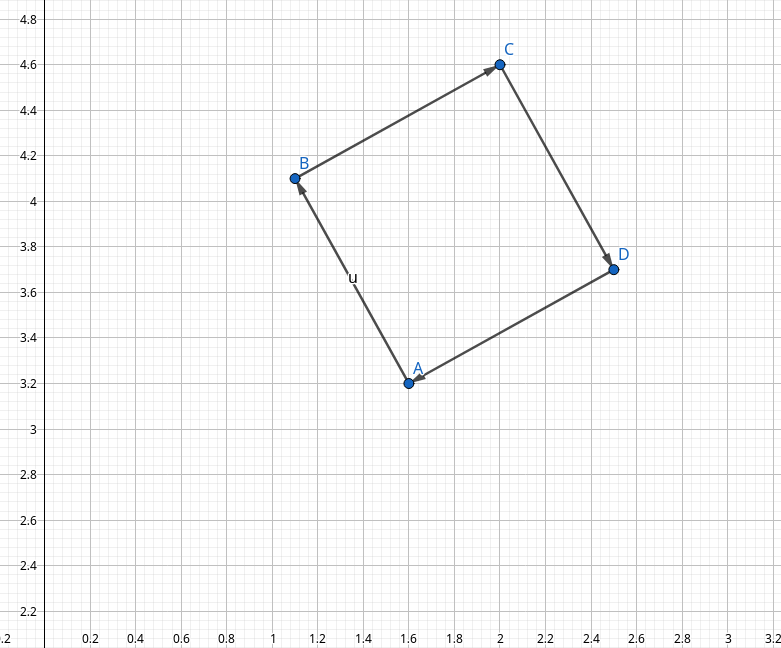
\includegraphics[width=0.7\textwidth]{images/8a_resp.png}
    \caption{Resultado do item 8a}
    \label{fig:8a_resp}
\end{figure}

\begin{enumerate}[label=\alph*), resume]
    \item Para o mesmo objeto da questão anterior, inverta a ordem das operações, ou seja faça primeiro a rotação e depois a translação. Construa a matriz de transformação e aplique ao objeto. Mostre graficamente a nova posição do objeto.
\end{enumerate}

Para realizar ambas transformações, precisamos realizar uma operação de composição. Então, $B$ sendo a transformação desejada, $R$ sendo a rotação e $T$ a translação, temos que:

\begin{gather*}
    \begin{bmatrix}
    x' \\
    y' \\
    1
    \end{bmatrix}
    = T \cdot R \cdot
    \begin{bmatrix}
    x \\
    y \\
    1
    \end{bmatrix} \\
    P' = B \cdot P \\
    B = T \cdot R
\end{gather*}

Assim, a composição fica:
\begin{equation*}
    \renewcommand\arraystretch{2}
    B = 
    \begin{bmatrix}
    1 & 0 & 3 \\
    0 & 1 & 2 \\
    0 & 0 & 1
    \end{bmatrix}
    \cdot
    \begin{bmatrix}
    \frac{\sqrt{3}}{2} & -\frac{1}{2} & 0 \\
    \frac{1}{2} & \frac{\sqrt{3}}{2} & 0 \\
    0 & 0 & 1
    \end{bmatrix}
    =
    \begin{bmatrix}
    \frac{\sqrt{3}}{2} & -\frac{1}{2} & 3 \\
    \frac{1}{2} & \frac{\sqrt{3}}{2} & 2 \\
    0 & 0 & 1
    \end{bmatrix}
\end{equation*}

As coordenadas do objeto da figura \ref{fig:8a} são (0,0), (0,1), (1,0), (1,1). Após a transformação, as coordenadas finais são (3, 2), (3.9, 2.5), (2.5, 2.9), (3.4, 3.4), arredondando para 1 casa decimal. O resultado pode ser visto na figura \ref{fig:8b_resp} abaixo:

\begin{figure}[H]
    \centering
    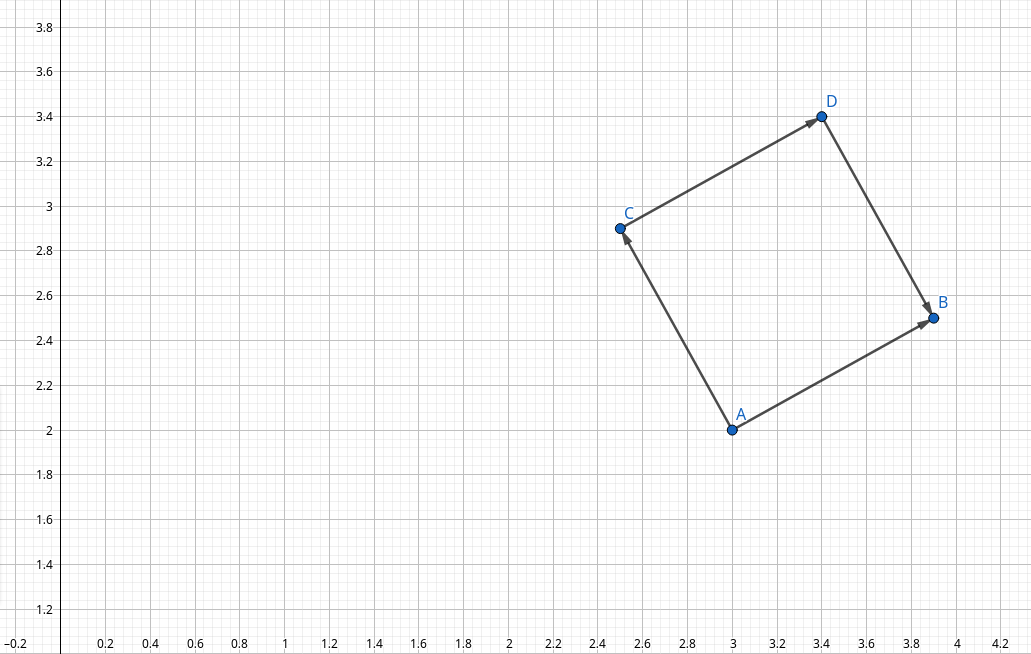
\includegraphics[width=0.8\textwidth]{images/8b_resp.png}
    \caption{Resultado do item 8b}
    \label{fig:8b_resp}
\end{figure}

\begin{enumerate}[label=\alph*), resume]
    \item O que pode concluir?
\end{enumerate}

Se pode concluir que, como as figuras resultantes de ambas composições não são iguais, translação e rotação não são transformações comutativas entre si. No primeiro resultado, a imagem está mais deslocada para cima, enquanto no segundo resultado a imagem está mais deslocada para a direita, e a diferença em ambos eixos é de aproximadamente 1.2 a 1.4.

\begin{enumerate}[label=\alph*), resume]
    \item Porque usamos coordenadas homogêneas para especificar transformações geométricas em CG?
\end{enumerate}

Usamos coordenadas homogêneas para melhor realizar composição de transformações com multiplicações entre matrizes. Sem elas, algumas transformações (como translação) não poderiam ser compostas com multiplicação.

% %%%%%%%%%%%%%%%%%%%
\section*{Questão 9}
% %%%%%%%%%%%%%%%%%%%
{\bfseries Dado três pontos (x(0), y(0)), (x(1), y(1)), (x(2), y(2)) no plano (x, y), mostre
como calcular uma matriz de coeficiente C (2 x 3) tal que 
\begin{equation*}
    q(t) =  
    \begin{bmatrix}
    x(t) \\
    y(t) 
    \end{bmatrix}
    = C
    \begin{bmatrix}
    t^2 \\
    t \\
    1
    \end{bmatrix}
\end{equation*}
a curva q(t) passa pelos três pontos dados em t = 0, 0.5, 1. Note que a curva q(t) é quadrática, em vez de cúbica.}

Como a curva é quadrática, temos que:
\begin{gather*}
    x(t) = a_xt^2 + b_xt + c_x \\
    y(t) = a_yt^2 + b_yt + c_y 
\end{gather*}{}

Assim, com os valores de $t$ que temos, podemos, para ambos eixos, encontrar sistema de 3 equações e 3 incógnitas. Primeiro, para o eixo x:
\begin{gather*}
    x(0) = c_x = x_0\\
    x(0.5) = \frac{a_x}{4} + \frac{b_x}{2} + c_x = x_1\\
    x(1) = a_x + b_x + c_x = x_2\\
\end{gather*}
Substituindo $c_x$ em todas as equações e multiplicando x(0.5) por 4, temos:
\begin{gather*}
    4x_1 = a_x + 2b_x + 4x_0\\
    x_2 = a_x + b_x + x_0
\end{gather*}{}

Subtraindo a segunda equação da primeira, conseguimos encontrar $b_x$:
\begin{gather*}
    4x_1-x_2 = b_x + 3x_0\\
    b_x = -3x_0 + 4x_1 - x_2 
\end{gather*}{}

Substituindo em x(1), conseguimos o último coeficiente $a_x$:
\begin{gather*}
    x_2 = a_x -3x_0 + 4x_1 - x_2 + x_0\\
    a_x = 2x_0 - 4x_1 + 2x_2
\end{gather*}{}

Assim, temos:
\begin{gather*}
    a_x = 2x_0 - 4x_1 + 2x_2\\
    b_x = -3x_0 + 4x_1 - x_2 \\
    c_x = x_0    
\end{gather*}{}

O processo é exatamente o mesmo para o eixo y, gerando o mesmo resultado, mas com $y_i, 0\leq i \leq 2$.

A matriz de coeficientes $C$ é da forma:
\begin{equation*}
    C=
    \begin{bmatrix}
    a_x & b_x & c_x \\
    a_y & b_y & c_y
    \end{bmatrix}
\end{equation*}

Considerando as equações para os coeficientes da primeira linha e seus análogos para y, temos:
\begin{equation*}
    C=
    \begin{bmatrix}
    2x_0 - 4x_1 + 2x_2 & -3x_0 + 4x_1 - x_2 & x_0 \\
    2y_0 - 4y_1 + 2y_2 & -3y_0 + 4y_1 - y_2 & y_0 
    \end{bmatrix}
\end{equation*}

% %%%%%%%%%%%%%%%%%%%
\section*{Questão 10}
% %%%%%%%%%%%%%%%%%%%
{\bfseries Defina exemplos de representações implícitas, explícitas e paramétricas de uma superfície. Quando consideramos uma imagem como uma função matemática bidimensional, podemos considerar a imagem como uma superfície? Em caso afirmativo, qual das três representações acima corresponde a uma imagem?}

Formas implícitas de uma superfície no espaço estão na forma $f(x,y,z) = 0$. Um exemplo seria uma esfera representada por $x^2 + y^2 + z^2 - r^2 = 0$, onde $r$ é o raio da esfera.

Formas explícitas de uma superfície no espaço são dadas na forma $z = f(x,y)$ ou equivalente. Um exemplo seria o plano $z = 3x+y$.

Formas paramétricas de uma superfície no espaço podem ser obtidas a partir das outras formas substituindo parâmetros $u,v$ para definirem a superfície. Por exemplo, no plano dado explicitamente, $z=3x+y$, podemos definir $u=x-1$ e $v=y+5$, e assim temos a curva paramétrica:
\begin{gather*}
    x(u,v) = u+1\\
    y(u,v) = v-5\\
    z(u,v) = 3u+v-2
\end{gather*}

Podemos considerar uma imagem como uma superfície, representando como função, na qual o eixo z é o valor de cada pixel, dado pela coordenada (x,y). A imagem, nesse caso, estaria na forma \textbf{explícita} de superfície $z = f(x,y)$.

% %%%%%%%%%%%%%%%%%%%
\section*{Questão 11}
% %%%%%%%%%%%%%%%%%%%
{\bfseries Defina a forma paramétrica da curva cúbica Bézier B(t) considerando os seguintes pontos de controle: $P0 = (1, 2)$, $P1 = (4, -1)$ e $P2 = (8, 6)$. Calcule as equações $(x(t), y(t))$ e obtenha o ponto B(0.5).}

Questão cancelada: faltando um ponto de controle.

% %%%%%%%%%%%%%%%%%%%
\section*{Questão 12}
% %%%%%%%%%%%%%%%%%%%
{\bfseries Uma curva cúbica Hermite passa através dos pontos (0,0), (2,4), (4,3), (5,-2) as quais estão parametrizadas em $t=[0,\frac{1}{4},\frac{3}{4},1]$, respetivamente. Determine a matriz de coeficientes C na qual C pode ser definida como (M*G).}

A curva cúbica Hermite fornece a matriz de coeficientes $C$, sendo que $C=MG$. Na curva de Hermite, $M$ é uma matriz definida a partir da inversa de uma matriz obtida pelo polinômio cúbico e a paramentrização, e $G$ é a matriz definida pelos pontos fornecidos:

\begin{gather*}
    P\left( 0 \right) = (0,0) \\
    P\left(\frac{1}{4}\right) = (2,4) \\
    P\left(\frac{3}{4}\right) = (4,3) \\
    P\left(1\right) = (5,-2) \\
    G =
    \begin{bmatrix}
    0 & 0 \\
    2 & 4 \\
    4 & 3 \\
    5 & -2
    \end{bmatrix}
\end{gather*}

O polinômio, para cada parâmetro, tem mesma equação para x e y. Assim, substituindo os valores de $t$ no polinômio cúbico, obtemos os coeficientes da matriz inversa de $M$, a matriz que, ao multiplicar $C$, gera os pontos dados:
\begin{equation*}
    \renewcommand\arraystretch{2}
    B =
    \begin{bmatrix}
    0 & 0 & 0 & 1 \\
    \frac{1}{64} & \frac{1}{16} & \frac{1}{4} & 1\\
    \frac{27}{64} & \frac{9}{16} & \frac{3}{4} & 1\\
    1 & 1 & 1 & 1
    \end{bmatrix}
\end{equation*}{}

A matriz $M$ é obtida ao obter a inversa de $B$.
\begin{equation*}
    \renewcommand\arraystretch{2}
    M=
    \begin{bmatrix}
    -\frac{16}{3} & \frac{32}{3} & -\frac{32}{3} & \frac{16}{3}\\ 
    \frac{32}{3} & -\frac{56}{3} & \frac{40}{3} & -\frac{16}{3}\\
    -\frac{19}{3} & 8 &-\frac{8}{3} & 1\\
    1 & 0 & 0 & 0
    \end{bmatrix}
\end{equation*}

Enfim, temos $C=MG$:

\begin{equation*}
    \renewcommand\arraystretch{2}
    C =
    \begin{bmatrix}
    -\frac{16}{3} & \frac{32}{3} & -\frac{32}{3} & \frac{16}{3}\\ 
    \frac{32}{3} & -\frac{56}{3} & \frac{40}{3} & -\frac{16}{3}\\
    -\frac{19}{3} & 8 &-\frac{8}{3} & 1\\
    1 & 0 & 0 & 0
    \end{bmatrix}
    \cdot
    \begin{bmatrix}
    0 & 0 \\
    2 & 4 \\
    4 & 3 \\
    5 & -2
    \end{bmatrix}
    =
    \begin{bmatrix}
    \frac{16}{3} & 0\\
    -\frac{32}{3} & -24\\
    \frac{31}{3} & 22\\
    0 & 0
    \end{bmatrix}
\end{equation*}{}

Temos então, que $P\left(t\right) = TC$, e ao realizar a multiplicação pode-se confirmar que a matriz está correta.

% %%%%%%%%%%%%%%%%%%%
\section*{Questão 13}
% %%%%%%%%%%%%%%%%%%%
{\bfseries Bônus: Defina a forma paramétrica da curva cúbica Hermite, dados os pontos bidimensionais $P1 = (0,0)$ e $P2 = (1,0)$ e os dois vetores tangentes $Pt1 = (1, 1)$ e $Pt2 = (0, -1)$.}

A curva cúbica Hermite fornece a matriz de coeficientes $C$, sendo que $C=MG$. Na curva de Hermite, $M$ é uma matriz definida a partir da inversa de uma matriz obtida pelo polinômio cúbico e sua derivada (vetores tangentes), e $G$ é a matriz definida pelos pontos extremos e os vetores tangentes fornecidos:

\begin{equation*}
    M = 
    \begin{bmatrix}
    2 & -2 & 1 & 1 \\
    -3 & 3 & -2 & -1\\
    0 & 0 & 1 & 0\\
    1 & 0 & 0 & 0
    \end{bmatrix}
\end{equation*}
\begin{equation*}
    G =
    \begin{bmatrix}
    0 & 0 \\
    1 & 0 \\
    1 & 1 \\
    0 & -1
    \end{bmatrix}
\end{equation*}

Assim, a matriz $C$ é dada por:
\begin{equation*}
    C = 
    \begin{bmatrix}
    2 & -2 & 1 & 1 \\
    -3 & 3 & -2 & -1\\
    0 & 0 & 1 & 0\\
    1 & 0 & 0 & 0
    \end{bmatrix}
    \cdot
    \begin{bmatrix}
    0 & 0 \\
    1 & 0 \\
    1 & 1 \\
    0 & -1
    \end{bmatrix}
    =
    \begin{bmatrix}
    -1 & 0 \\
    1 & -1 \\
    1 & 1 \\
    0 & 0
    \end{bmatrix}
\end{equation*}

A forma paramétrica da curva pode ser encontrada multiplicando os termos do polinômio com essa matriz ($P(t) = TMG = TC$).
\begin{equation*}
    P(t)=
    \begin{bmatrix}
    t^3 & t^2 & t & 1
    \end{bmatrix}
    \cdot
    \begin{bmatrix}
    -1 & 0 \\
    1 & -1 \\
    1 & 1 \\
    0 & 0
    \end{bmatrix}
    =
    \begin{bmatrix}
    -t^3 + t^2 + t & -t^2+t 
    \end{bmatrix}
\end{equation*}

Assim, temos que a curva paramétrica é:
\begin{gather*}
    x(t) = -t^3 + t^2 + t\\
    y(t) = -t^2 + t
\end{gather*}

\end{document}